\section{Теоретическая часть}

\subsection{Введение}
Стационарный электрический ток в замкнутой цепи может существовать благодаря источникам тока, в которых на заряженные частицы (носители тока) действуют сторонние непотенциальные силы $\vec{F}_{\text{ст}}$. Электродвижущей силой (ЭДС) на участке цепи 1--2 называется работа сторонней силы, совершаемая при перемещении по этому участку единичного положительного заряда:
\begin{align} \label{eq:1}
	\mathcal{E}_{12} = \int_{1}^{2} \vec{E}_{\text{ст}} d\vec{l},
\end{align}
где $\vec{E}_{\text{ст}}$ -- напряженность поля сторонних сил.

Сторонние силы могут иметь различную природу. Так, например, в химических источниках тока стороннее силовое поле возникает в тонких контактных слоях между электродами и электролитом.

Под действием сторонних сил происходит разделение зарядов, в результате чего возникает кулоновское поле $\vec{E}_{\text{кул}}$. Работа кулоновской силы при перемещении единичного положительного заряда есть разность потенциалов:
\begin{align} \label{eq:2}
	\varphi_1 - \varphi_2 = \int_{1}^{2} \vec{E}_{\text{кул}} \cdot d\vec{l}.
\end{align}

Кроме сторонних и кулоновских сил на носители тока действуют силы сопротивления. Поскольку алгебраическая сумма работ всех сил равна нулю, на любом участке цепи выполняется закон Ома:
\begin{align} \label{eq:3}
	I R_{12} = \varphi_1 - \varphi_2 + \mathcal{E}_{12}.
\end{align}

\subsection{Измерение ЭДС при помощи вольтметра}
\begin{figure}[H]
	\centering
	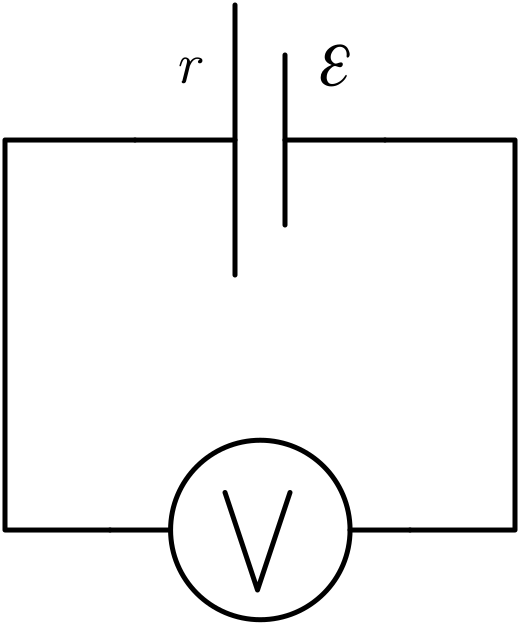
\includegraphics[width=0.3\linewidth]{graph1}
	\caption{Измерение ЭДС при помощи вольтметра.}
	\label{fig:1}
\end{figure}
При подключении вольтметра с сопротивлением $R_v$ к батарее, имеющей ЭДС $\mathcal{E}$ и внутреннее сопротивление $r$ (\Cref{fig:1}), показания вольтметра:
\begin{align} \label{eq:4}
	U = I R_v = \frac{\Epsilon R_v}{R_v + r}.
\end{align}

Показания вольтметра отличаются от значения $\mathcal{E}$ на величину
\begin{align}
	\mathcal{E} - U = I r = \frac{\mathcal{E} r}{R_v + r}.
\end{align}



При $R_v \gg r$ относительная ошибка измерения ЭДС становится малой:
\begin{align} \label{eq:6}
	\delta\mathcal{E} = \frac{\Epsilon - U}{\Epsilon} = \frac{\Epsilon r}{\Epsilon (R_v + r)} = \frac{r}{R_v + r} \approx \frac{r}{R_v}.
\end{align}

Для высокоомных вольтметров эта ошибка может быть незначительной, но для невысокоомных вольтметров измерение дает заметную погрешность. Более точное измерение обеспечивает метод компенсации.

\subsection{Метод компенсации}
Для пояснения идеи метода компенсации рассмотрим схему, приведенную на \cref{fig:2}.

\begin{figure}[H]
	\centering
	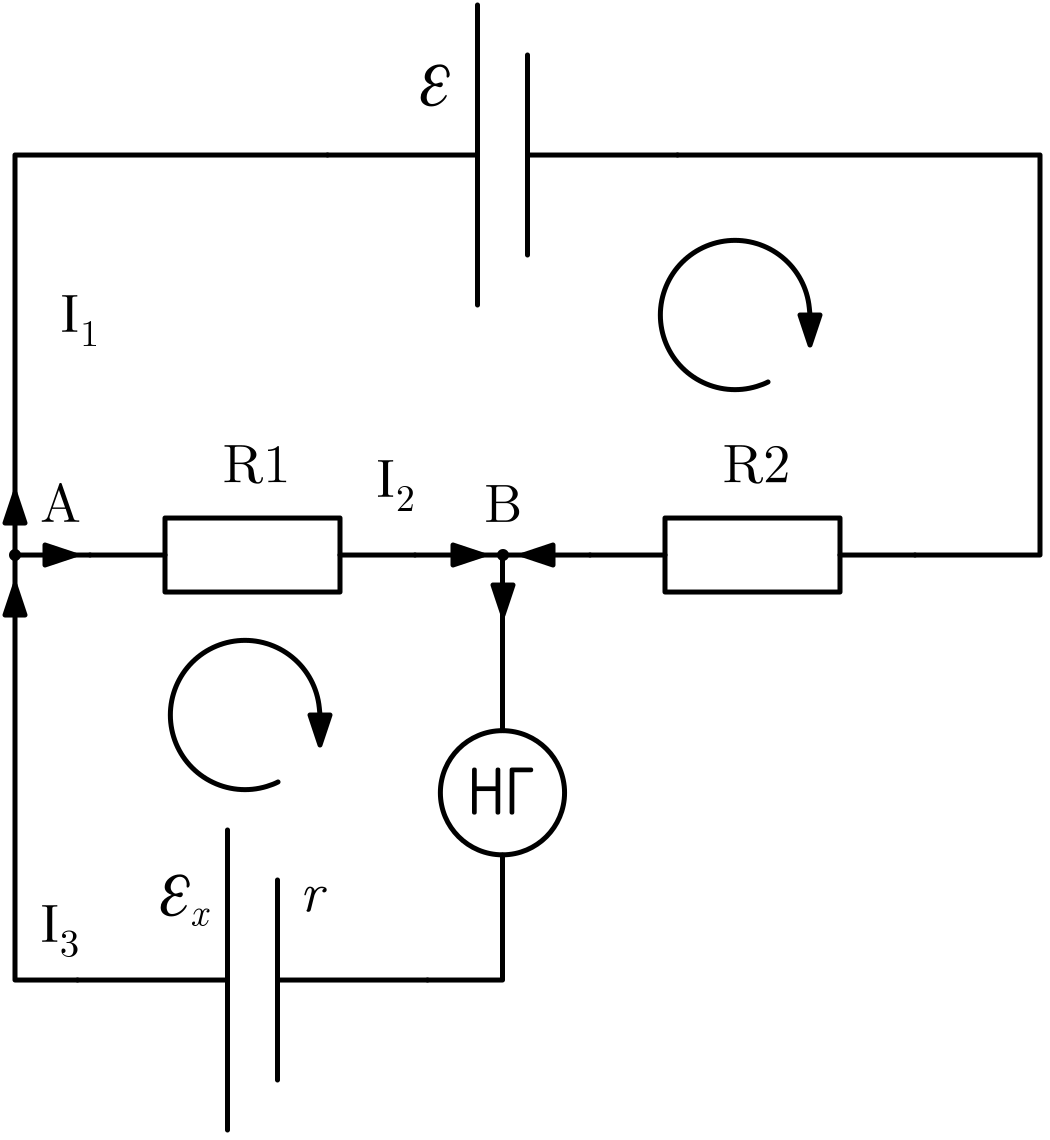
\includegraphics[width=0.7\linewidth]{graph2}
	\caption{Принципиальная схема измерения ЭДС методом компенсации.}
	\label{fig:2}
\end{figure}

Здесь $\mathcal{E}_x$ -- неизвестная ЭДС, $\mathcal{E}$ -- ЭДС источника питания ($\mathcal{E} > \mathcal{E}_x$). Методика измерения состоит в подборе сопротивления $R_1$ при неизменной сумме
\begin{align} \label{eq:7}
	R_1 + R_2 = R = \text{const},
\end{align}
до достижения нулевого тока через нуль-гальванометр. 

Для получения тока через гальванометр, рассмотрим \cref{fig:2} и расставим направления течения тока и обхода. Запишем первый и второй законы Кирхгофа:
\begin{align} \label{eq:1.1}
	\begin{cases}
		I_3 = I_1 + I_2\\
		-\Epsilon_x = I_3 r + I_2 R_1\\
		\Epsilon = I_1 R_2 - I_2 R_1
	\end{cases}
\end{align}

Выведем силу тока на промежутке с нуль гальванометре ($I_3$):
\begin{align}\label{eq:1.2}
	\begin{cases}
		I_3 = I_1 + I_2\\
		I_2 = \dfrac{\Epsilon_x}{R_1} - I_3 \dfrac{r}{R_1}\\
		I_1 = I_2 \dfrac{R_1}{R_2} - \dfrac{\Epsilon}{R_2} = \left(\dfrac{\Epsilon_x}{R_1} - I_3 \dfrac{r}{R_1}\right) \dfrac{R_1}{R_2} - \dfrac{\Epsilon}{R_2} = \dfrac{\Epsilon_x - \Epsilon}{R_2} - I_3 \dfrac{r}{R_2}
	\end{cases}
\end{align}
\[I_3 = \dfrac{\Epsilon_x - \Epsilon}{R_2} - I_3 \dfrac{r}{R_2} + \dfrac{\Epsilon_x}{R_1} - I_3 \dfrac{r}{R_1}\]
\[I_3 \left(1 + \dfrac{r}{R_2} + \dfrac{r}{R_1}\right) = \dfrac{\Epsilon_x - \Epsilon}{R_2} + \dfrac{\Epsilon_x}{R_1}\]
\[I_3 \dfrac{r R + R_1 R_2}{R_1 R_2} = \dfrac{R_1 \Epsilon - R \Epsilon_x}{R_1 R_2}\]
\begin{align} \label{eq:8}
	I_3 = \frac{\mathcal{E} R_1 - \mathcal{E}_x R}{rR + R_1 R_2}.
\end{align}

При компенсации ($I_3 = 0$) неизвестная ЭДС:
\[0 = \mathcal{E} R_{1x} - \mathcal{E}_x R\]
\begin{align} \label{eq:9}
	\mathcal{E}_x = \frac{R_{1x}}{R} \mathcal{E},
\end{align}
где $R_{1x}$ -- значение $R_1$ при компенсации.

Чтобы исключить $\mathcal{E}$ из расчетов, проводят измерение с эталонной ЭДС $\mathcal{E}_N$:
\begin{align} \label{eq:10}
	\mathcal{E}_N = \frac{R_{1N}}{R} \mathcal{E}.
\end{align}

Из \eqref{eq:9} и \eqref{eq:10} получаем:
\begin{align} \label{eq:11}
	\mathcal{E}_x = \frac{R_{1x}}{R_{1N}} \mathcal{E}_N.
\end{align}

Таким образом, для измерения $\mathcal{E}_x$ необходимо определить два значения сопротивления $R_1$ при компенсации. ЭДС источника питания знать не требуется.

\subsection{Экспериментальная установка}

Рабочая схема для измерения ЭДС методом компенсации приведена на \cref{fig:3}.

В качестве источника питания используется блок питания БП-28, эталонной ЭДС -- нормальный элемент НЭ-65. Резисторы $R_1$ и $R_2$ -- два одинаковых штепсельных магазина с постоянной суммой $R = R_1 + R_2$.

Защитный резистор $R_3$ предохраняет нормальный элемент и гальванометр от больших токов. Перед измерениями $R_3$ вводят полностью, а при приближении к компенсации уменьшают до нуля.

Схема включается ключом $K_2$ с последовательным замыканием цепей для защиты приборов. Сначала замыкается цепь питания, затем подключается ветвь с измеряемой ЭДС.

\begin{figure}[b]
	\centering
	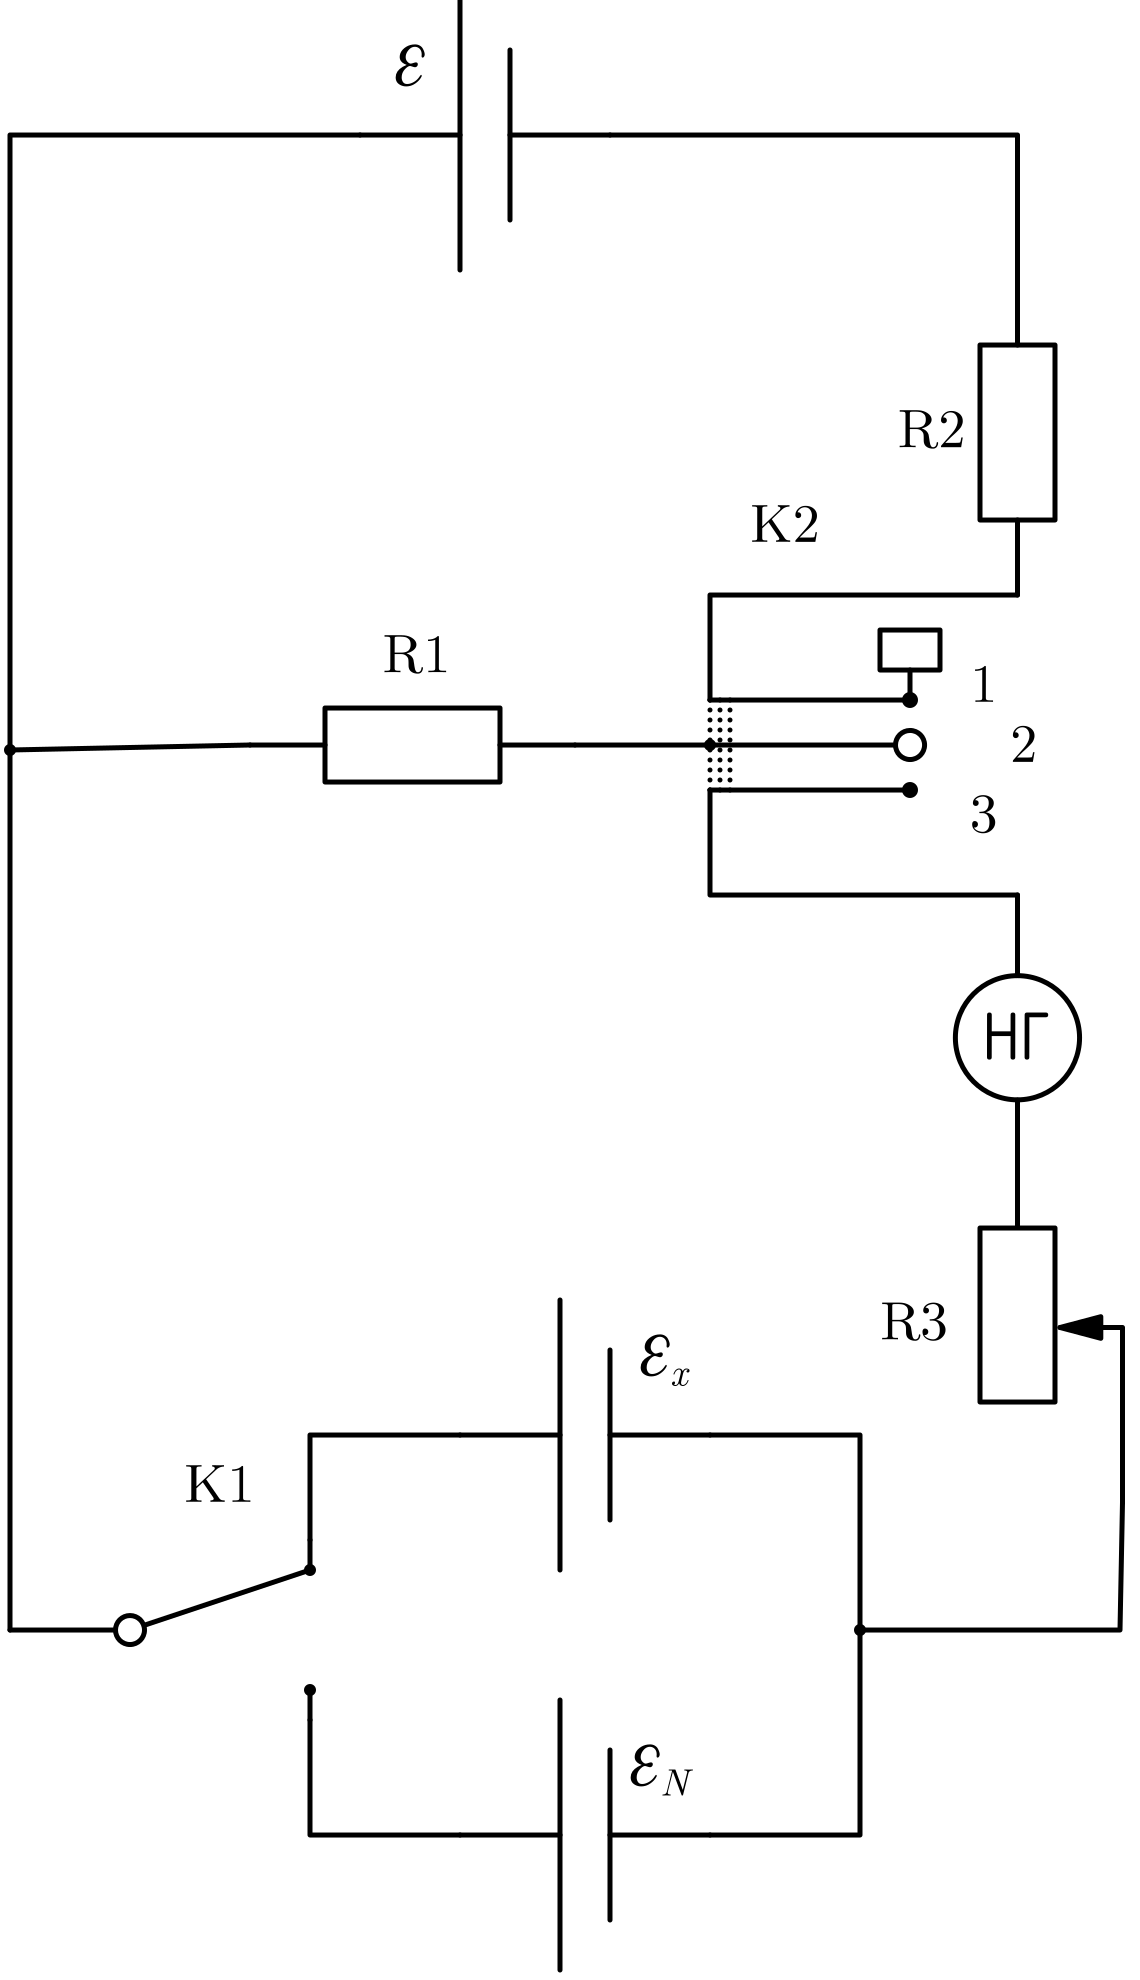
\includegraphics[width=0.8\linewidth]{graph3}
	\caption{Рабочая схема для определения ЭДС методом компенсации}
	\label{fig:3}
\end{figure}